
% !TeX program = pdflatex
\documentclass[11pt,a4paper]{article}
\usepackage[utf8]{inputenc}
\usepackage[T1]{fontenc}
\usepackage[turkish]{babel}
\usepackage{lmodern}
\usepackage{geometry}
\usepackage{graphicx}
\usepackage{float}
\usepackage[section]{placeins}
\usepackage{flafter}
\usepackage{caption}
\usepackage{subcaption}
\usepackage{booktabs}
\usepackage{siunitx}
\usepackage{hyperref}
\usepackage{longtable}
\usepackage{xcolor}
\usepackage{microtype}
\usepackage{etoolbox}
\usepackage{amsmath,amssymb}
\usepackage[most]{tcolorbox}
\usepackage{enumitem}

% --- Sayfa düzeni ---
\geometry{margin=1.3cm}
\hypersetup{colorlinks=true,linkcolor=blue,citecolor=blue,urlcolor=blue}
\graphicspath{{../results/}}
\setkeys{Gin}{width=1\linewidth, keepaspectratio}

% --- Kutu stilleri ---
\tcbset{
  colback=gray!3,
  colframe=gray!60!black,
  boxrule=0.4pt,
  arc=2pt,
  left=6pt,right=6pt,top=6pt,bottom=6pt
}
\newtcolorbox{info}[1][]{title={#1}}
\newtcolorbox{tipbox}{colback=blue!3,colframe=blue!60!black,title={Açıklama}}
\newtcolorbox{gloss}{colback=orange!3,colframe=orange!60!black,title={Kavram}}

% --- Başlık bilgisi ---
\title{NPM Ekosisteminde Yönlü Karmaşık Ağ Analizi \\
\large Öğretici ve Akademik Genişletilmiş Sürüm}
\author{\textbf{Yusuf Talha ARABACI}}
\date{\today}

\begin{document}
\maketitle

\begin{abstract}
Bu belge, NPM ekosistemindeki bağımlılık ilişkilerini ağ bilimi yaklaşımıyla inceleyen bir çalışmanın öğretici versiyonudur. Amaç, yazılım paketleri arasındaki yapısal ilişkilerin nasıl modellenebileceğini, ağ ölçümlerinin ne anlama geldiğini ve bu ölçümlerden elde edilen sonuçların sistemik risk açısından nasıl yorumlanabileceğini öğrenci düzeyinde açıklamaktır. 
\end{abstract}

\clearpage

\section{Giriş: Yazılım Ekosistemlerinde Bağımlılık ve Risk}
Modern yazılım geliştirme süreçlerinde bir proje nadiren sıfırdan yazılır; çoğu zaman binlerce hazır bileşen (paket) birbirine bağımlı şekilde kullanılır. Bu durum geliştirmenin hızını artırsa da, sistemin kırılganlığını da artırır.

\begin{tipbox}
Bir paketteki hata veya kötü niyetli değişiklik, ona bağımlı olan tüm projelere yayılabilir. Bu zincirleme yayılım, \textbf{tedarik zinciri riski} olarak adlandırılır.
\end{tipbox}

NPM (Node Package Manager) ekosistemi JavaScript dünyasında bu bağımlılık ilişkilerinin en yoğun olduğu alanlardan biridir. Çalışmamızın amacı, bu ekosistemi bir ağ (network) olarak düşünmek ve yapısal riskleri matematiksel olarak gözlemlemektir.

\section{Temel Kavramlar ve Kuramsal Arka Plan}
Bu bölümde ağ teorisinin temel kavramları sade bir dille açıklanmıştır.

\begin{gloss}
\textbf{Düğüm (Node):} Her bir paket, ağda bir noktadır. \\
\textbf{Kenar (Edge):} İki paket arasındaki “bağımlı $\to$ bağımlılık” yönlü bağlantısıdır.
\end{gloss}

\subsection{Yönlü Ağ}
Bir paket başka bir pakete bağımlıysa, bu ilişki yönlü bir bağ ile gösterilir. Örneğin:
\begin{center}
\texttt{A $\to$ B} demek, “A paketi B’ye bağımlıdır” anlamına gelir.
\end{center}

\subsection{In-Degree ve Out-Degree}
\begin{itemize}
  \item \textbf{In-degree:} Bu pakete kaç farklı paket bağımlı? (Popülerlik ve yayılım potansiyelini gösterir.)
  \item \textbf{Out-degree:} Bu paket kaç farklı pakete bağımlı? (Kırılganlık ve maruziyet düzeyini gösterir.)
\end{itemize}

\begin{tipbox}
Yüksek \textbf{in-degree} = “Birçok kişi bunu kullanıyor.” \\
Yüksek \textbf{out-degree} = “Bu paket çok şeye bağımlı, biri bozulursa etkilenir.”
\end{tipbox}

\subsection{Betweenness Merkeziyeti}
Ağda iki nokta arasındaki en kısa yolların kaç tanesi bu paketten geçiyor? Bunu ölçer. 
\begin{tipbox}
Bir paketin betweenness değeri yüksekse, o paket ağda \emph{köprü} konumundadır. Silinirse iki grup arasındaki bağlantı kopar.
\end{tipbox}

\subsection{Bileşik Risk Skoru}
Çeşitli metriklerin (in-degree, out-degree, betweenness) normalleştirilip birleştirilmesiyle elde edilir:
\[\text{Risk}(n) = 0.5\,\tilde d_{in}(n) + 0.2\,\tilde d_{out}(n) + 0.3\,\tilde b(n)\]
Böylece her paket için 0 ile 1 arasında bir risk değeri hesaplanabilir.

\section{Veri Toplama ve Yöntem}
\subsection{Veri Kaynakları}
NPM API ve npms.io servislerinden alınan paket verileriyle, her paketin bağımlılık listesi çıkarılmıştır.

\subsection{Ağ Kurulumu}
Elde edilen veriler Python’un \texttt{NetworkX} kütüphanesi ile yönlü bir graf yapısına dönüştürülmüştür. Her düğüm bir paketi, her kenar bir bağımlılığı temsil eder.

\subsection{Ölçümlerin Hesaplanması}
\begin{itemize}
  \item Her düğüm için in-degree, out-degree ve betweenness değerleri hesaplanır.
  \item Bu değerler min–max yöntemiyle 0–1 aralığına normalize edilir.
  \item Ağırlıklı ortalama alınarak bileşik risk skoru bulunur.
\end{itemize}

\begin{info}[Min–Max Normalizasyon]
Bir sayıyı 0–1 aralığına getirmek için şu formül kullanılır:
\[\tilde{x} = \frac{x - x_{\min}}{x_{\max} - x_{\min}}\]
Böylece tüm değişkenler aynı ölçeğe getirilir.
\end{info}

\subsection{Sağlamlık Analizi}
Yüksek riskli birkaç düğüm (paket) ağdan çıkarıldığında ağın bağlantı durumu tekrar ölçülür. 
Amaç, ağın kırılganlığını (robustluk düzeyini) gözlemlemektir.

\begin{tipbox}
Bir ağda birkaç kritik düğüm silindiğinde bile ağ bağlantısı korunabiliyorsa, o ağ \textbf{sağlamdır}. Ancak NPM ağı bu konuda zayıf görünmektedir.
\end{tipbox}

\section{Bulguların Görselleştirilmesi ve Yorumlanması}

\subsection{Ağın Genel Görünümü}
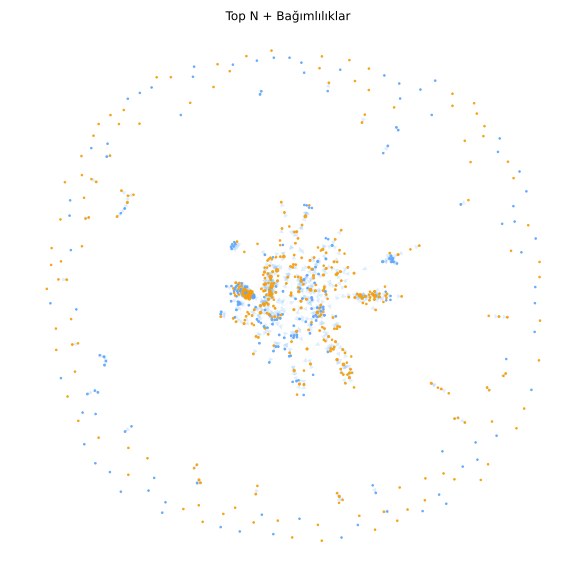
\includegraphics{network_full_topN.png}
\captionof{figure}{NPM paketleri arasındaki bağlantı ağı. Turuncular çekirdek (Top~N) paketleri gösterir.}
\begin{tipbox}
Merkezdeki büyük düğümler en çok kullanılan paketlerdir. Bu düğümler ağın omurgasını oluşturur.
\end{tipbox}

\subsection{Derece Dağılımları}
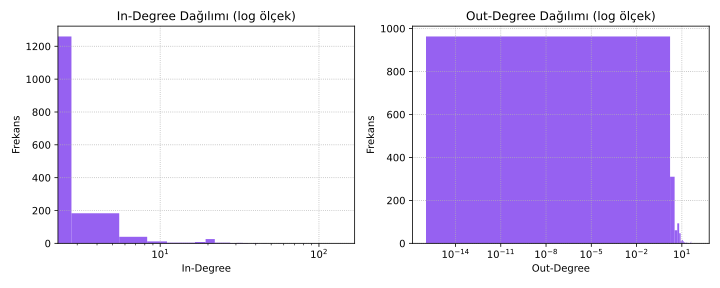
\includegraphics{degree_histograms.png}
\captionof{figure}{In-degree ve Out-degree dağılımları (log ölçek).}
\begin{tipbox}
Az sayıda çok büyük değere sahip paket vardır (örneğin Babel, TypeScript). Bu, ekosistemin dengesizliğini gösterir.
\end{tipbox}

\subsection{Korelasyon Analizi}
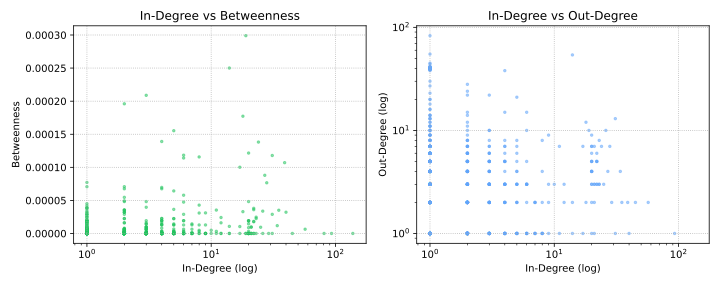
\includegraphics{scatter_correlations.png}
\captionof{figure}{Metrikler arası ilişkiler (in-degree–betweenness ve in-degree–out-degree).}
\begin{tipbox}
Popüler (yüksek in-degree) paketler genellikle ağda köprü (yüksek betweenness) rolü de oynar.
\end{tipbox}

\subsection{Risk Skorları}
\includegraphics{top20_risk.png}
\captionof{figure}{Bileşik risk skoruna göre en riskli 20 paket.}
\IfFileExists{../results/risk_scores_top20.tex}{\begin{longtable}{lrrrrr}
\caption{Top 20 Risk Skoru}\\
\toprule
Paket & Risk & In-Degree & Out-Degree & Betweenness & TopN? \\
\midrule
\endfirsthead
\toprule
Paket & Risk & In-Degree & Out-Degree & Betweenness & TopN? \\
\midrule
\endhead
\bottomrule
\endfoot
\bottomrule
\endlastfoot
tslib & 0.500000 & 138 & 0 & 0.000000 & True \\
es-abstract & 0.431785 & 14 & 54 & 0.000250 & True \\
get-intrinsic & 0.392937 & 19 & 10 & 0.000299 & True \\
@smithy/types & 0.339366 & 93 & 1 & 0.000000 & True \\
@babel/helper-plugin-utils & 0.293478 & 81 & 0 & 0.000000 & True \\
@aws-sdk/credential-provider-node & 0.271994 & 18 & 12 & 0.000177 & True \\
@aws-sdk/core & 0.261914 & 31 & 13 & 0.000118 & True \\
call-bound & 0.253485 & 39 & 2 & 0.000107 & True \\
@aws-sdk/nested-clients & 0.245554 & 4 & 38 & 0.000139 & False \\
@jest/types & 0.242459 & 24 & 7 & 0.000138 & True \\
side-channel & 0.232483 & 3 & 5 & 0.000209 & True \\
jest-snapshot & 0.224549 & 5 & 21 & 0.000155 & True \\
@puppeteer/browsers & 0.220782 & 2 & 7 & 0.000196 & False \\
@aws-sdk/types & 0.217789 & 57 & 2 & 0.000006 & True \\
jest-util & 0.208899 & 20 & 6 & 0.000122 & True \\
telecom-mas-agent & 0.203623 & 1 & 83 & 0.000000 & True \\
call-bind & 0.195697 & 27 & 4 & 0.000088 & True \\
@smithy/smithy-client & 0.195157 & 28 & 7 & 0.000077 & True \\
debug & 0.179578 & 40 & 1 & 0.000032 & True \\
@babel/traverse & 0.178945 & 17 & 7 & 0.000100 & True \\
\end{longtable}
}{\fbox{risk\_scores\_top20.tex bulunamadı}}
\begin{tipbox}
En riskli paketler genellikle altyapı düzeyindeki küçük ama çok kullanılan modüllerdir (\texttt{es-abstract}, \texttt{tslib}, \texttt{babel}, vb.).
\end{tipbox}

\subsection{Kaskad Etkisi}
\includegraphics{cascade_impact_top20.png}
\captionof{figure}{Riskli paketlerin neden olabileceği zincirleme etki boyutu.}
\IfFileExists{../results/cascade_impact_top20.tex}{\input{../results/cascade_impact_top20.tex}}{\fbox{cascade\_impact\_top20.tex bulunamadı}}
\begin{tipbox}
Bazı küçük paketler beklenmedik derecede çok sayıda başka paketi etkileyebilir — bu, ağın karmaşıklığının sonucudur.
\end{tipbox}

\subsection{Sağlamlık Deneyi}
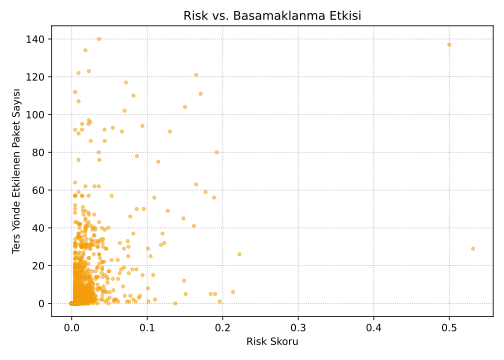
\includegraphics{risk_vs_cascade.png}
\captionof{figure}{Risk skoru ve kaskad etkisi arasındaki ilişki.}
\begin{tipbox}
İlişki doğrusal değildir. Bu, yalnızca bir metriğe bakarak sistemik riski anlamanın yetersiz olduğunu gösterir.
\end{tipbox}


\subsection{Köprü Kenarlar (Edge Betweenness)}
\IfFileExists{../results/edge_betweenness_top10.tex}{\begin{longtable}{l l r}
\caption{Edge Betweenness Ilk 10 (Yuksek kopru kenarlar)}\\
\toprule
U & V & Edge Betweenness \\
\midrule
\endfirsthead
\toprule
U & V & Edge Betweenness \\
\midrule
\endhead
\bottomrule
\endfoot
\bottomrule
\endlastfoot
jest & @jest/core & 0.000142 \\
@jest/expect & jest-snapshot & 0.000100 \\
reflect.getprototypeof & which-builtin-type & 0.000094 \\
@jest/transform & babel-plugin-istanbul & 0.000086 \\
@babel/traverse & @babel/generator & 0.000082 \\
jest-snapshot & @jest/transform & 0.000081 \\
call-bound & get-intrinsic & 0.000081 \\
@babel/core & @babel/helper-compilation-targets & 0.000078 \\
telecom-mas-agent & jest & 0.000077 \\
jest-snapshot & babel-preset-current-node-syntax & 0.000076 \\
\end{longtable}
}{\fbox{edge\_betweenness\_top10.tex bulunamadı}}
\begin{tipbox}
Köprü kenarlar, alt ağları birbirine bağlayan kırılgan bağlantılardır. Bu bağlar koptuğunda ağ parçalanabilir.
\end{tipbox}
\section{Tartışma ve Değerlendirme}
Bu analiz NPM ekosisteminde ağın aşırı merkezî olduğunu göstermiştir. 
Az sayıda paket ekosistemin çok büyük kısmını birbirine bağlamaktadır.

\begin{itemize}
  \item \textbf{Avantaj:} Yönetim kolaylığı, yeniden kullanım.
  \item \textbf{Dezavantaj:} Yüksek sistemik risk ve kırılganlık.
\end{itemize}

\begin{tipbox}
Bir paketin bozulması yüzlerce projenin etkilenmesine yol açabilir. Bu nedenle güvenlik yalnızca kod düzeyinde değil, ağ düzeyinde de incelenmelidir.
\end{tipbox}


\subsection{Ağın Temel İstatistikleri}
\IfFileExists{../results/graph_stats.tex}{\input{../results/graph_stats.tex}}{\fbox{graph\_stats.tex bulunamadı}}
\begin{tipbox}
Düğüm ve kenar sayıları ölçeği; bileşen sayısı parçalanma seviyesini; en büyük bileşen çekirdeğin büyüklüğünü gösterir.
\end{tipbox}
\section{Sınırlamalar ve Geliştirme Alanları}
\begin{itemize}
  \item Veriler yalnızca \texttt{dependencies} alanına dayalıdır, peer bağımlılıklar hariçtir.
  \item Betweenness hesaplaması örnekleme yöntemiyle yapılmıştır.
  \item Ağın görsel düzeni sezgiseldir; yerleşim algoritmaları sonucu etkileyebilir.
\end{itemize}

\section{Sonuç ve Öğrenilenler}
Bu çalışma, ağ biliminin yazılım güvenliği bağlamında nasıl kullanılabileceğini göstermektedir. 
Öğrenciler için çıkarılabilecek dersler şunlardır:

\begin{enumerate}
  \item Yazılım güvenliği sadece kod taraması değil, \textbf{bağımlılık yapısının} incelenmesini de gerektirir.
  \item Ağ analizi araçları (\texttt{NetworkX}, \texttt{Gephi}, vb.) bu tür karmaşık ilişkileri anlamada etkilidir.
  \item “Küçük ama merkezi” paketlerin önemi, sistemik risk açısından büyüktür.
\end{enumerate}

\appendix
\section*{Ek A: Temel Terimler Sözlüğü}
\begin{longtable}{@{}p{0.25\linewidth}p{0.7\linewidth}@{}}
\toprule
\textbf{Terim} & \textbf{Açıklama ve Örnek}\\
\midrule
In-degree & Bu paketi kaç proje kullanıyor? Örn: \texttt{tslib} birçok proje tarafından kullanılır.\\
Out-degree & Bu paket kaç farklı pakete bağımlı? Örn: \texttt{react-scripts} onlarca modüle bağlıdır.\\
Betweenness & Ağdaki iki nokta arasındaki yolların ne kadarında bu paket var?\\
Kaskad Etkisi & Bir paketteki hatanın dolaylı olarak etkileyebileceği diğer paket sayısı.\\
Bileşik Risk Skoru & Yukarıdaki metriklerin ağırlıklı birleşimi (0–1 arası).\\
\bottomrule
\end{longtable}

\end{document}
